\setlength\abovedisplayskip{0.4pt}
\setlength\belowdisplayskip{0.4pt}

\chapter{Measuring luminosity}

Although the analysis results presented in this thesis do not require a precise knowledge of the measured luminosity, it is important to introduce it since the author contributed in this direction. 

\section{Instantaneous luminosity}

One of the most important quantities measured by CMS is luminosity. Luminosity is necessary to convert the number of events detected, for a given channel into a collision cross section. Collision cross-sections are among the primary observables predicted by theoretical physicists. For particle physics, the collision cross-section of a process is typically measured through the relation:
\begin{equation}
\sigma  = \frac{R}{\mathit{L}} ,
\end{equation}
where $\sigma$ is the cross section, $R$ is the rate at which the process occurs per collision, and $L$ is the instantaneous luminosity. $L$ is measured via the rate of a given luminometer and taking into account the acceptance $A$
\begin{equation}
L  = \frac{R}{ \sigma_{o}(E) A(t,\mu,n_b,...)} ,
\end{equation}
The denominator is typically measured as the visible cross section, $\sigma_{vis}$,
\begin{equation}
\sigma_{vis}  = \sigma_{o}(E) A(t,\mu,n_b,...),
\end{equation}
where $\sigma_{o}(E)$ comes from separating out the dependence of $\sigma_{vis}$ on collision energy E. $\sigma_{vis}$ ideally has no dependence on time or experiment conditions, i.e. constant with respect to pile-up and invariant to filling scheme. For example activity in the HF scales with the instantaneous luminosity. Therefore, the visible cross-section -- which has no time dependence -- can be used as calibration constant for converting the rate of HF activity into instantaneous luminosity. Every luminometer should have its own characteristic visible cross section. In this way, multiple independent luminometers can cross check each other \cite{CMS:2013gfa,cmsLumi,Krasny:2006xg}.

\section{Luminometers}

Within CMS, the Beam Radiation and Luminosity (BRIL) group is responsible for providing luminosity measurements and studying the radiation levels for the various detectors. There are two kinds of CMS luminometer: online and offline. Online luminometers readout the luminosity per bunch in real time. As of 2015 there are three online luminometers: the pixel luminosity telescope (PLT), the HF, and the beam conditions monitor (BCM1f). There is a high-rate, independent data-acquisition system for each of the online luminometers. Offline luminometers measure the rate of reconstructed objects. The primary offline lumimoneter is the pixel tracker. In general, the offline lumimometers have better stability over time. \cite{CMS:2010gua}

The online and offline luminometers complement each other for high precision data analysis. Specifically, the offline data can be used to calibrate out imperfections in the online data. 

In addition to these hardware luminometers, CMS can use physics processes as luminosity benchmarks.  For example, the measured the Z-boson cross-section to a high accuracy and high precision is an alternative.

\subsection{Pixel cluster counting}

One of the primary methods of measuring instantaneous luminosity is through pixel cluster counting (PCC) in the pixel-tracker. The collision rate is linked to instantaneous luminosity $L$ via the total inelastic cross-section $\sigma_T$
\begin{equation}
v \mu  = L \sigma_T,
\end{equation}
where $v=11246$ Hz is the beam revolution frequency and $\mu$ is the number of collisions per bunch crossing. We define the average number of pixel clusters per event, $\left \langle n \right \rangle$, as
\begin{equation}
\left \langle n \right \rangle = \mu n_1,
\end{equation}
and the visible cross section $\sigma_{vis}$ as 
\begin{equation}
\sigma_{vis} = \sigma_T n_1,
\end{equation}
where $n_1$ is the average number of pixel clusters per inelastic collision. Leveraging the previous two equations, the instantaneous luminosity reduces to
\begin{equation}
L = \frac{v\left \langle n \right \rangle}{\sigma_{vis}},
\end{equation}
such that $L$ can be calculated after measuring the actual $\left \langle n \right \rangle$ of the data \cite{CMS:2013gfa}

\subsection{Pixel luminosity telescope}

The pixel luminosity telescope (PLT) is one of the online luminometers of CMS. The PLT consists of 8 pixel telescopes arranged around the beamline on either side of the CMS interaction point. Each telescope has three layers of silicon pixel detector. Triple coincidences in these telescopes are measured as luminosity on a bunch-by-bunch basis. As an independent luminomemter, the PLT data is also useful for reducing the systematic uncertainty of the luminosity delivered to CMS. 

\begin{figure}[]
\begin{centering}
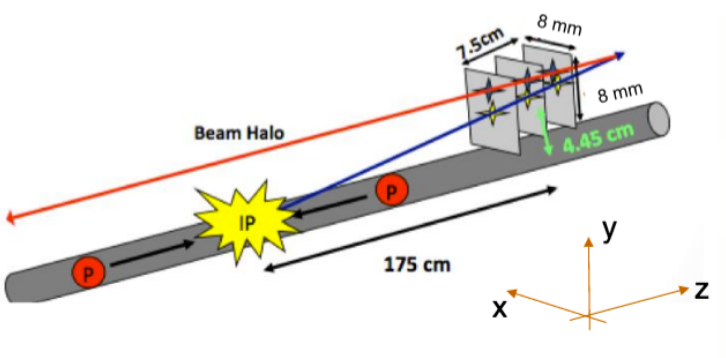
\includegraphics[width=5in]{Chapter4/importfigs/plt_triple.png}
\par\end{centering}
\caption{PLT triple coincidence \label{fig:pltTriple}}
\end{figure}

The PLT was installed as part of the CMS Run-2 upgrades. The hardware of the pixel sensors and the readout chip are similar to those used by the pixel tracker. However, the readout chips (ROC) of the PLT are capable of delivering fast-OR formatted data; the pixel tracker cannot do this. The fast-OR readout is optimized for delivering triple-coincidence data; whereas the standard pixel data readout has a maximum frequency of 100 kHz, the PLT fast-OR readout maxes out at an orders of magnitude greater frequency, at 40 Mhz \cite{Kornmayer:2016wkz}.

\subsection{Hadronic forward calorimeter}

As mentioned before in section 3.2.3.1, the hadronic forward calorimeter (HF) of CMS is capable of measuring luminosity. Because of the high flux of particles through the forward region, the HF-luminosity is less subject to statistical uncertainty than the PCC-luminosity. The HF can measure luminosity per bunch through its own dedicated high-rate acquisition system (HTR) that is separate from the CMS DAQ. Within the HF, the HTR boards each have an additional HF luminosity transmition circuit (HLX). The HLX are mounted in one of the mezzanine expansion slots of the HTR.

The HF luminosity is subject to two difficulties. Because the PMTs require a calibrated voltage, the accumulation of gain changes over long periods of time will cause calibration drifts. Furthermore, the HF detector response has been shown to be nonlinear with respect to vertex pile-up. Substantial data analysis goes into calculating the corrections to these two sources of error \cite{CMS:2013gfa}.  

\subsection{Fast Beam Conditions Monitor}

The CMS Beam Conditions and Radiation Monitoring System (BRM) provides a wide variety of information on the accumulated radiation dosage into CMS. This information is essential for protecting CMS from radiation damage. There are many subcomponents to the BRM system, one of which is the Fast Beam Conditions Monitor (BCM1F). The BCM1F is capable of measuring the beam-halo background and the flux from collision products. Similar to the PLT, BCM1F is located close to the beam pipe; however, BCM1F uses diamonds instead of silicon pixels. The readout from BCM1F is not digital, but an analog signal sent through optical fibres. 

There are 24 single crystal diamond sensors in the BCM1F system. The BCM1F is located very close to interaction point, specifically 1.8 m on either side. This location is chosen specifically to take advantage of the 25 ns between bunch crossings. From the BCM1F vantage point there is a 12.5 ns delay between particle fluxes from the machine induced background and those coming from actual collisions. Thus the BCM1F can use timing to distinguish between signal and background \cite{Guthoff:2017ibf}.  

\section{Van de Meer scanning calibration}

The luminometers of CMS produce signals proportional to the instantanteous luminosity of the LHC beam. However, these signals need to be properly calibrated with respect to a known visible cross-section for each luminometer. This calibration is accomplished via Van de Meer scanning \cite{vanderMeer:1968zz}. The opposing beams of LHC are moved back and forth in the transverse plane. During the scan, the detector response is measured as a function of beam displacement. The beam widths are calculated from Gaussian fits to the detector response. The visible cross-section of the luminometer in question is then derived from the width of the beams, and acts as the calibration of the detector response. Figure \ref{fig:pccVdMScans} presents the fitting of the VdM scan in the X and Y planes \cite{CMS:2013gfa}. The visible cross section, in terms of VDM scan variables, is 
\begin{equation}
\sigma_{vis} = \frac{2 \pi \Sigma_x \Sigma_y v\left \langle n \right \rangle_{\Delta=0}}{N_1 N_2},
\end{equation}
where $\Sigma_x \Sigma_y$ is the beam overlap, $v$ is the revolution frequency, $\left \langle n \right \rangle_{\Delta=0}$ is the amplitude of the VDM rate profile, and $N_1 N_2$ is the product of the number of protons (or heavy-ions) in the beams.

\begin{figure}[]
\begin{centering}
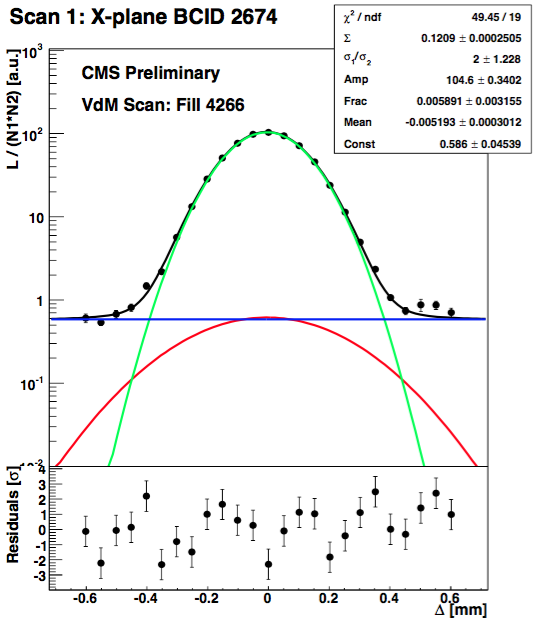
\includegraphics[width=3in]{Chapter4/importfigs/CMS-PAS-LUM-15-001_Figure_005-a.png}
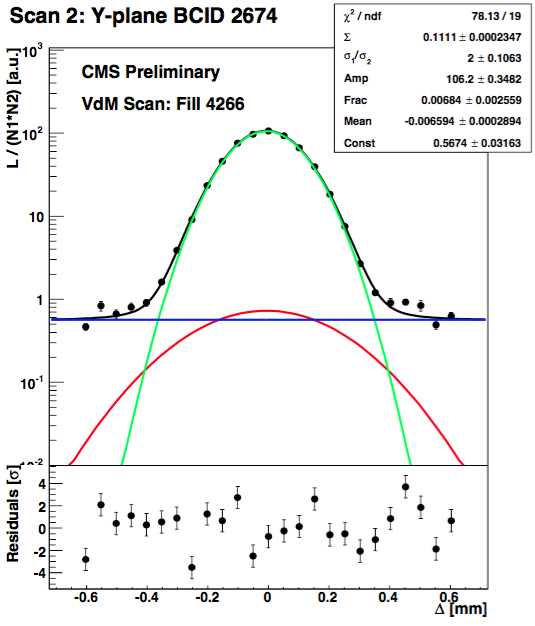
\includegraphics[width=3in]{Chapter4/importfigs/CMS-PAS-LUM-15-001_Figure_005-b.png}
\par\end{centering}
\caption{PCC VdM Scans \cite{CMS:2013gfa} \label{fig:pccVdMScans}}
\end{figure}

\section{Corrections to VDM scans}

Several corrections must be applied to VdM scan data before calculating the visible cross section. These corrections are considered uncorrelated, i.e. it does not matter in what order they are applied. The results of the VDM scan must be corrected for the following phenomena: the length scale, the ghosts and satellite background, the growth in beam emittance, orbit drift, and beam-beam electromagnetic effects. These affect the normalization of the VDM scans, and so the corrections take the form of calibration constants derived from additional scans and beam monitoring subdetectors \cite{CMS:2013gfa}. 

The length scale correction is derived by comparing the effects of a length scan to the response of the tracker; checking the difference between the reported beam displacement and that seen in the tracker. In addition to the circulating bunches, the LHC beams can be polluted by foreign particles that were not intended for injection by LHC commissioning. The presence of these foreign particles -- fleeting "ghosts" and persistent "satellites" -- can be detected by comparing the total beam current, measured by the DC beam current transformer, against the per bunch current measured by the Fast Beam Current Transformers (FBCT). The FBCT, because it is timed for bunch crossings, is less likely to interact with ghosts and satellites. Variations in beam emmitance affect the VdM scans by changing the amplitude and width of the rate profile. The orbit drift correction is based on data from the Beam Position Monitors (BPM), which measure the position of the beam orbit in LHC. Lastly, beam-beam effects refer to the electromagnetic forces that the beams exert on each other; for example, when the beams are transversely separated there is a small, but statistically significant, induced magnetic force. 

\section{Systematic uncertainty}

Table \ref{fig:sysLumiError} displays the systematic uncertainties associated with the delivered luminosity. The "normalization" uncertainties are for the visible cross section, $\sigma_{vis}$. The "integration" uncertainties are for the integrated luminosity that is calculated using the $\sigma_{vis}$. The stability uncertainty is calculated from comparing the relative contributions of pixel tracker layers to total number of pixel clusters measured in a span of time. From run to run, each pixel layer contribution varies by no more than 1\%. It is possible for the rate of high track multiplicity events to exceed the temporary storage capacity of the tracker read-out buffer; the resulting inefficiencies are mainly found in the first barrel layer of the tracker. The "afterglow" refers to background noise associated with electrical excitations in the detector material, and warrants a correction factor to the integrated luminosity. 

\begin{table}[]
\begin{centering}
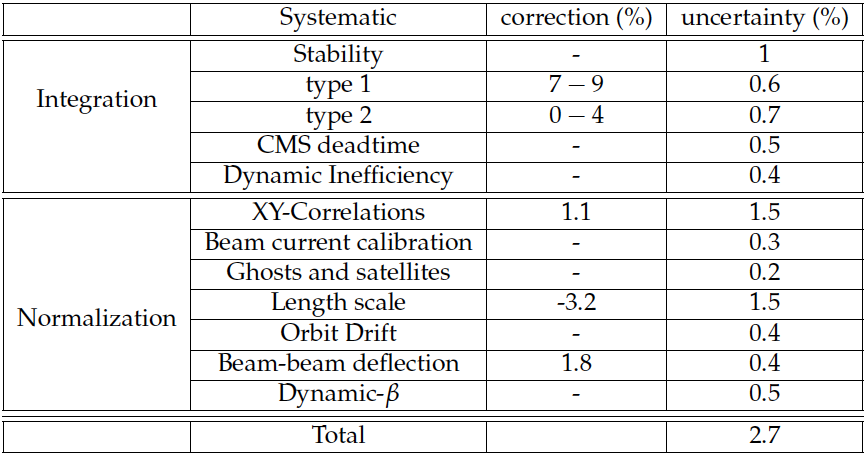
\includegraphics[width=4in]{Chapter4/importfigs/CMS-PAS-LUM-15-001_Table_001.png}
\par\end{centering}
\caption{Systematic uncertainty during the 2015 pp run \cite{CMS:2013gfa}. \label{fig:sysLumiError}}
\end{table}


\section{Author's contributions}

The 2015 heavy-ion run itself recorded about $1.4 pb^-1$ in integrated luminosity. This integrated luminosity is reconstructed into data on the order of pentabytes. Table \ref{fig:lumiFill} presents LHC the 2015 PbPb run luminosity information, and presents for each fill the peak instantaneous luminosity, delivered integrated luminosity, and recorded integrated luminosity. The last column, EffbyLumi, is the ratio of the delivered to recorded integrated luminosities.  

\begin{table}[h!]
\begin{centering}
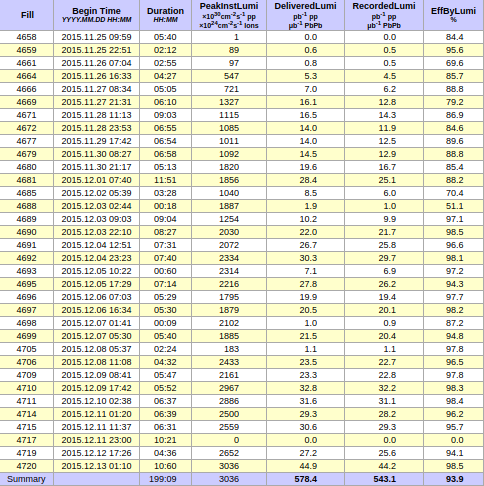
\includegraphics[width=5.5in]{Chapter4/importfigs/lumiFill.png}
\par\end{centering}
\caption{Luminosity by CMS fill. \label{fig:lumiFill}}
\end{table}

I contributed to CMS luminosity validation and performed studies on the long-term stability of the BRIL luminometers. On a week by week basis, I would examine the data from online and offline luminometers and certify that it met the quality standards of CMS. If the data exhitibed non-linear behavior, I would de-certify the corresponding lumi-sections in the BRIL files, which are in the JSON format.

All CMS data has to go through a data certification workflow. Data certification insures that only valid data is used in CMS analyses. Decisions on data certification are recorded in two systems: the DQM Run Registry, shown here in Figure \ref{fig:runRegistry}, and the normtag JSON files of the BRIL group. There are occasions when the sub-detectors of CMS might record poor quality data. For example, the software reading out data from the PLT could crash and thus compromise the output. In this case the certification workers would record the lumi sections during which the PLT software crashed. These lumi sections would be removed from the certifying JSON file passed on to the BRIL group. If all the luminometers are malfunctioning, a whole run could be invalidated in the run registry.

\begin{figure}[h!]
\begin{centering}
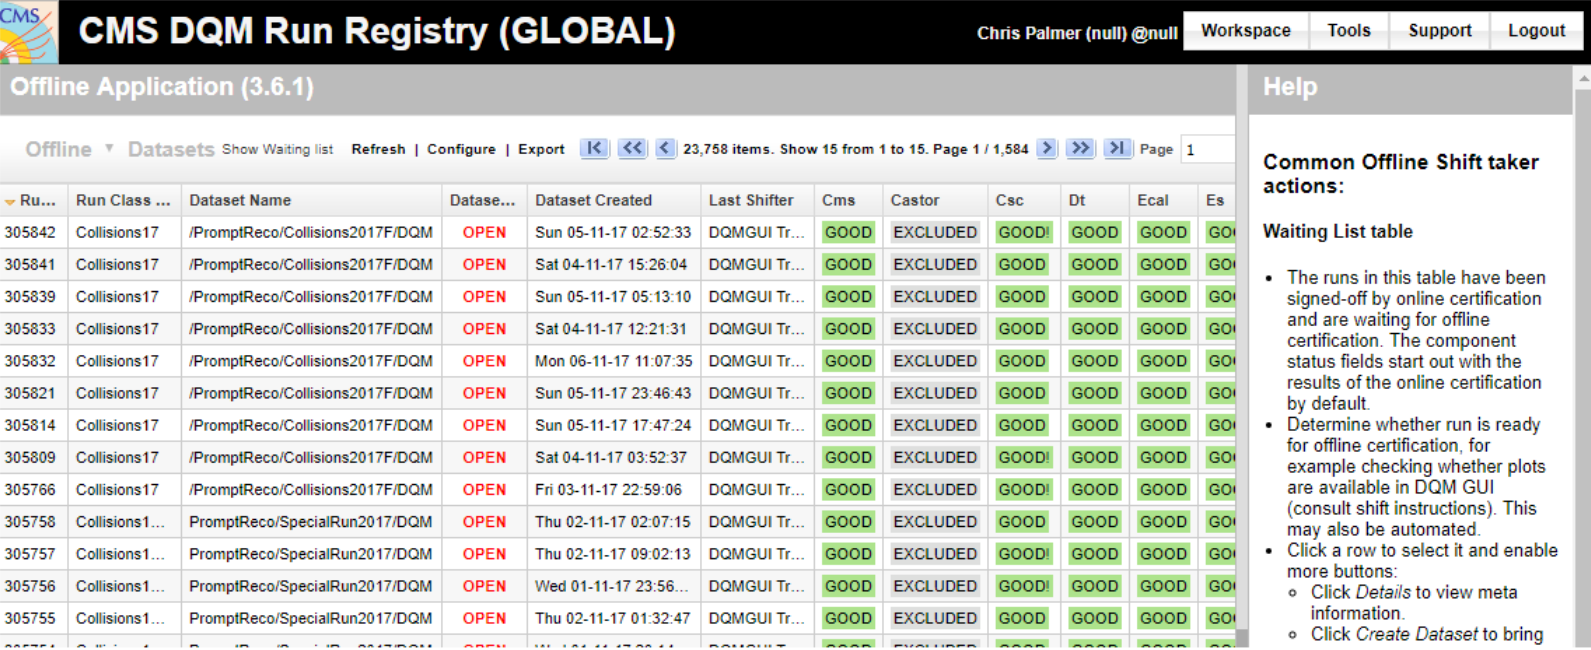
\includegraphics[width=6in]{Chapter4/importfigs/chris_palmer_run_registry.png}
\par\end{centering}
\caption{CMS Run Registry. \label{fig:runRegistry}}
\end{figure}

In additon to data certification, I reviewed the long-term stability of the BRIL luminometers during the 2015 and 2016 proton-proton runs. Stability refers to the comparative performance of the different luminometers. Ideally, the ratio of the instantaneous luminosity reported by separate luminometers should be a constant ratio, but in fact there is a tendency for this ratio to drift as a result of radiation damage to the luminometers. This drift can be seen in plotting the average ratio as a function of interaction rate and of the different measures of LHC time: runs, lumi-sections, and bunch-crossings.  Instantaneous luminosity, in theory, should be independent of machine conditions like acceptance and efficiency. Figure \ref{fig:lumiHi2015} is records the sum of the delivered and recorded integrated luminosity for each day of the 2015 Pb-Pb run. 

\begin{figure}[h!]
\begin{centering}
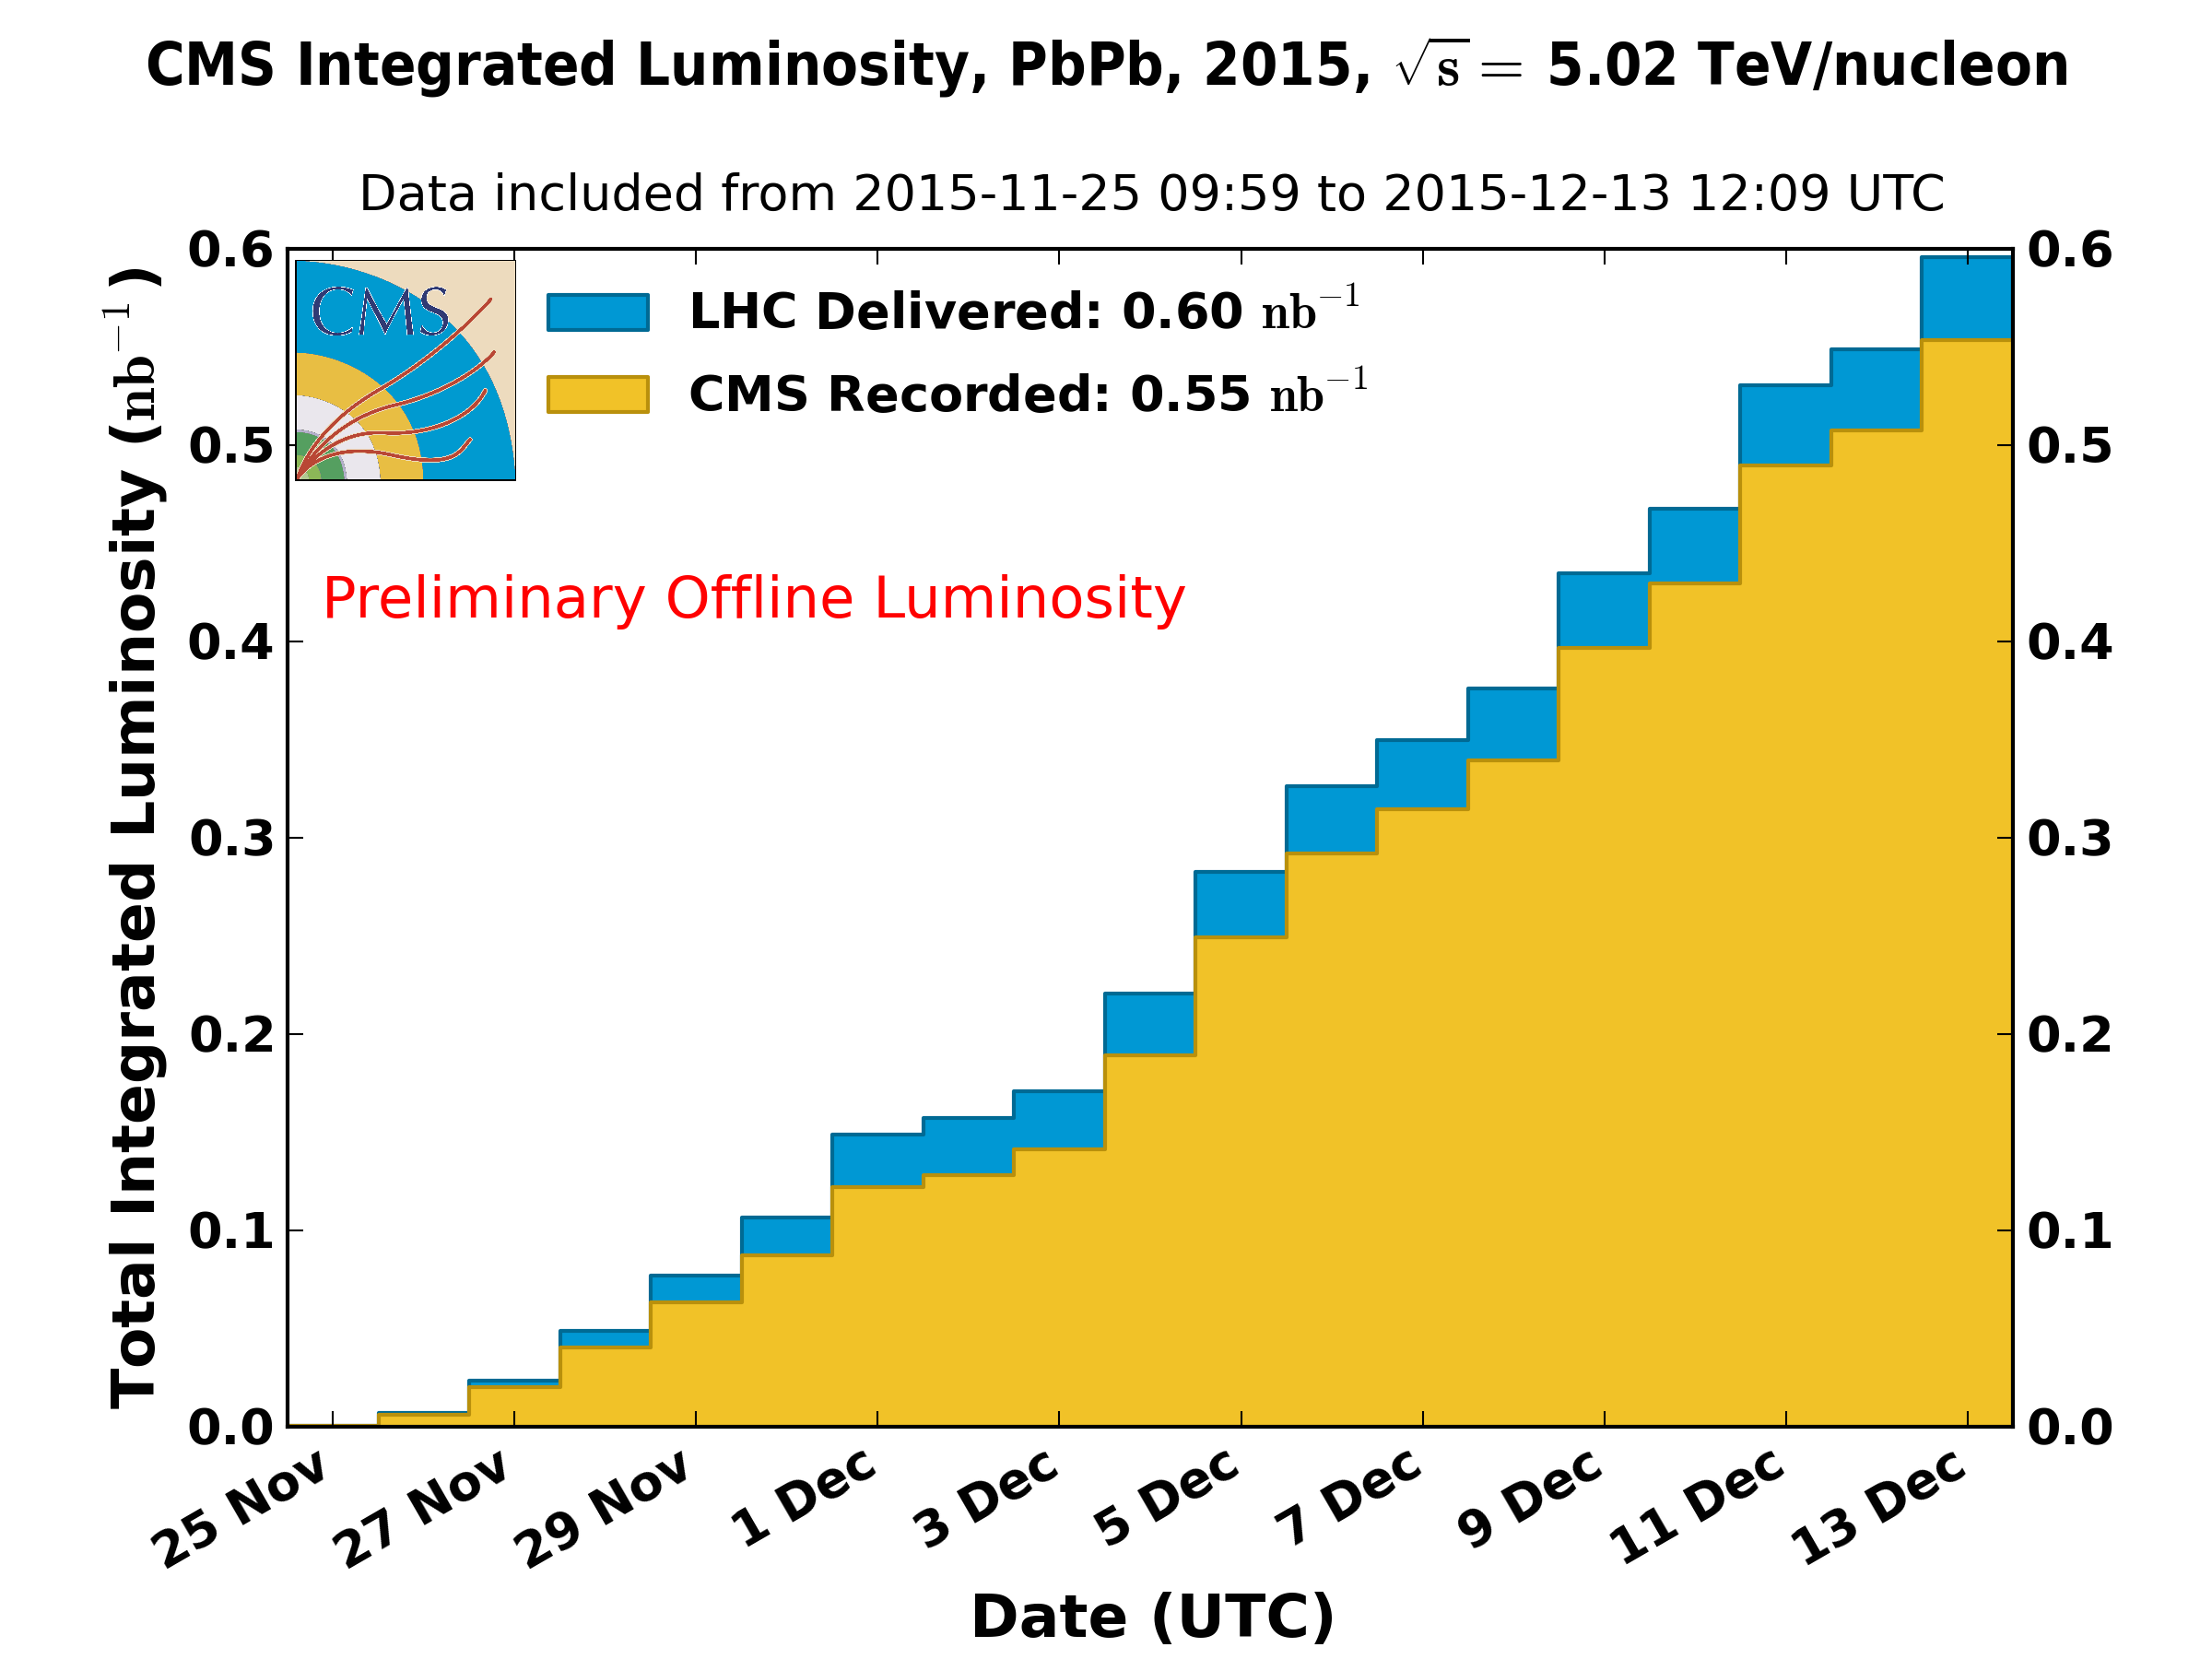
\includegraphics[width=5in]{Chapter4/importfigs/int_lumi_per_day_cumulative_pbpb_2015_pbpb.png}
\par\end{centering}
\caption{CMS lumi during the 2015 PbPb run. \label{fig:lumiHi2015}}
\end{figure}

Figure \ref{fig:lumiCMSEra} is the CMS-recorded integrated luminosity for each proton-proton era of LHC. Notice that as the collision energy increases, the recorded luminosity grows at steeper and steeper rate. This acceleration in the recorded luminosity is consistent with the higher multiplicity of high energy collisions. As LHC pushes the energy frontier, high quality luminosity analyses will become even more fundamental for the continued performance of CMS. The "High Luminosity Large Hadron Collider" (HL-LHC) is a project to increase the design luminosity of LHC by an order of magnitude by 2025. To fully leverage the power of this increased luminosity, particularly for studying possible anomalous couplings, CMS must continue providing measures of luminosity with tightly controlled systematic uncertainty. 

\begin{figure}[h!]
\begin{centering}
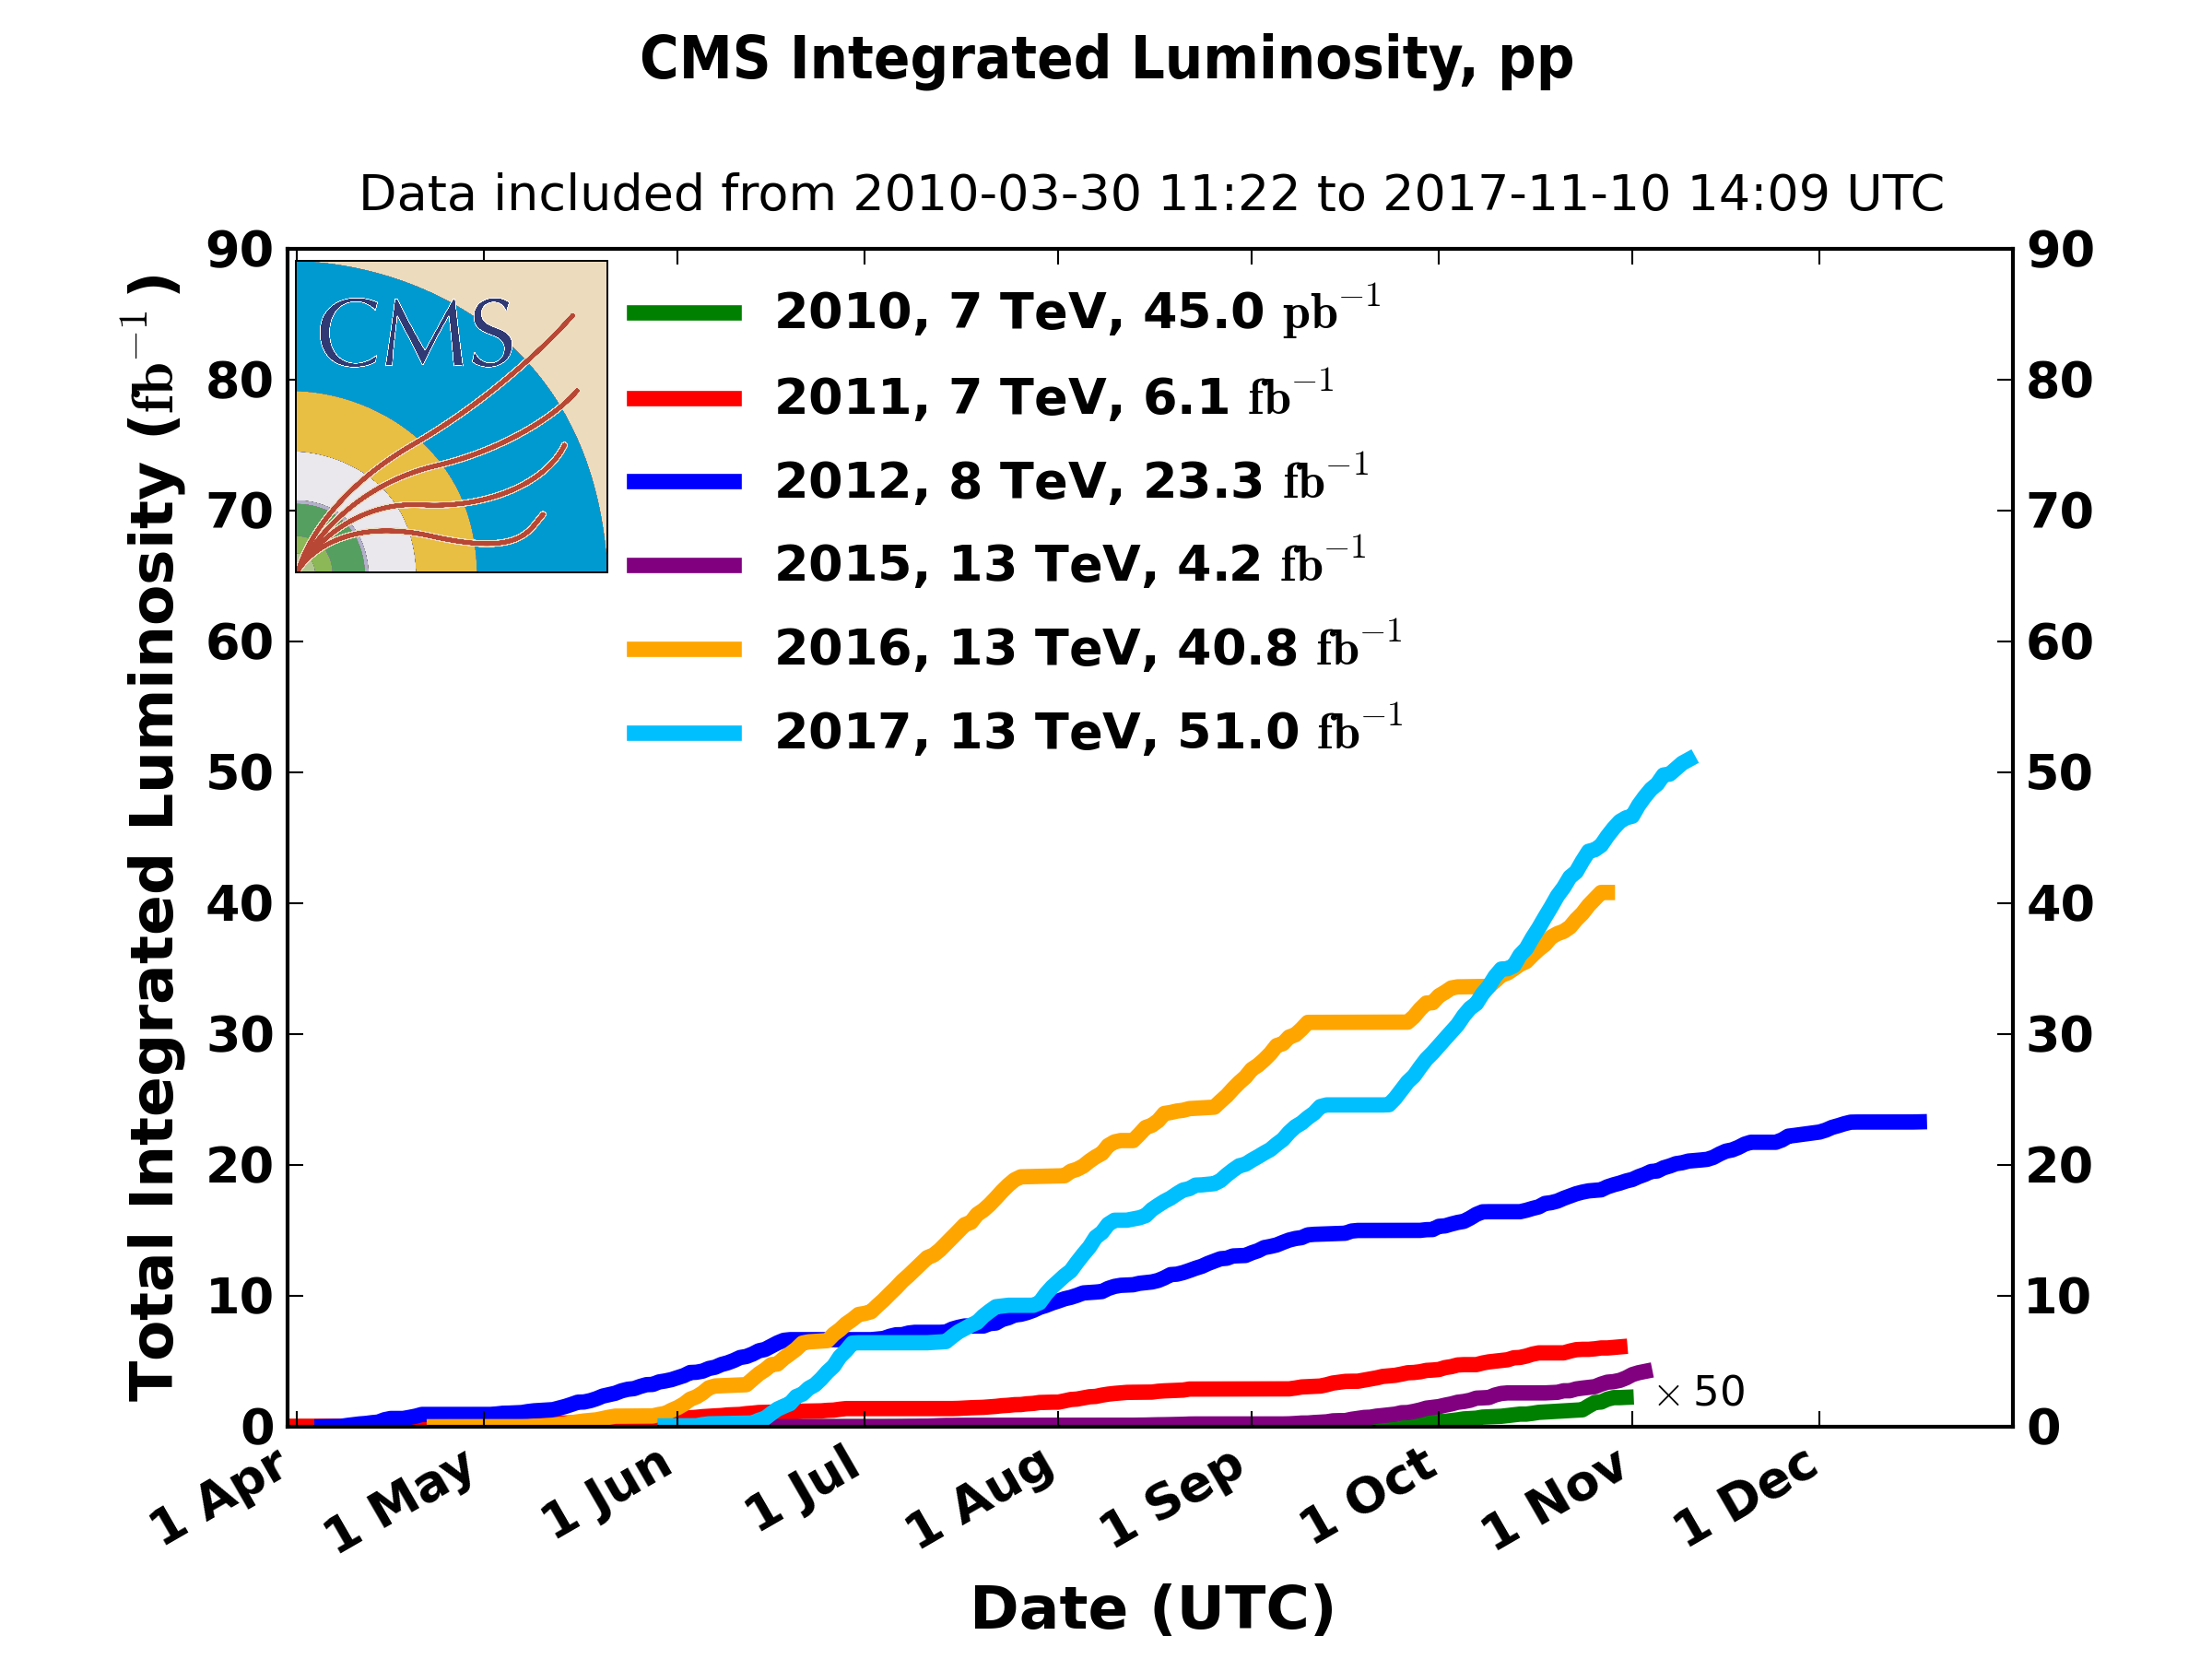
\includegraphics[width=5in]{Chapter4/importfigs/int_lumi_cumulative_pp_2.png}
\par\end{centering}
\caption{Total integrated luminosity for the various pp periods in 2010 until 2017. \label{fig:lumiCMSEra}}
\end{figure}